\begin{pastexam}[label={px:ntu-108-dsaa-09}]{臺大資工所 108 學年度 第 9 題}
（問答）

(10\%) At 9am, 14 ships are leaving for the other side as shown below, where the English
alphabets mean the types of those ships. For safety reasons, each ship can only stop at a pier
having the same alphabet, and, if the routes of two ships cross each other, one ship needs to wait
15 minutes before leaving.

\begin{center}
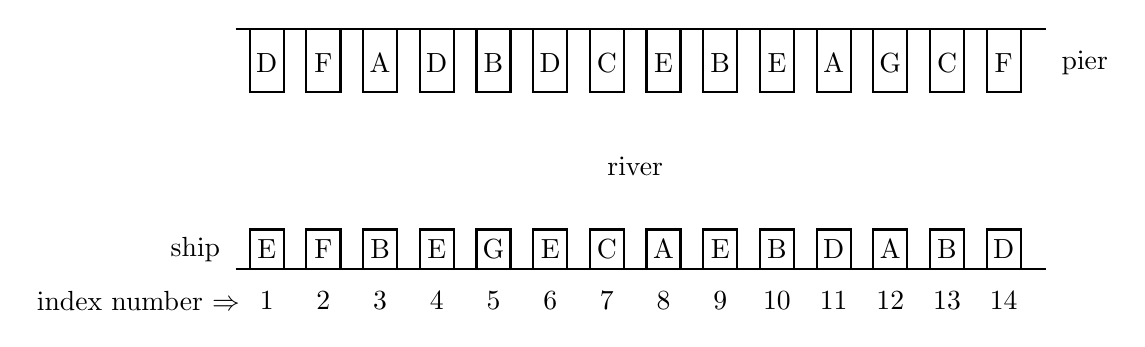
\begin{tikzpicture}[x=0.72cm,y=1cm]
\draw[thick] (0.45,3.05) -- (14.75,3.05);
\draw[thick] (0.70,2.25) rectangle (1.30,3.05); \node at (1,2.62) {D};
\draw[thick] (1.70,2.25) rectangle (2.30,3.05); \node at (2,2.62) {F};
\draw[thick] (2.70,2.25) rectangle (3.30,3.05); \node at (3,2.62) {A};
\draw[thick] (3.70,2.25) rectangle (4.30,3.05); \node at (4,2.62) {D};
\draw[thick] (4.70,2.25) rectangle (5.30,3.05); \node at (5,2.62) {B};
\draw[thick] (5.70,2.25) rectangle (6.30,3.05); \node at (6,2.62) {D};
\draw[thick] (6.70,2.25) rectangle (7.30,3.05); \node at (7,2.62) {C};
\draw[thick] (7.70,2.25) rectangle (8.30,3.05); \node at (8,2.62) {E};
\draw[thick] (8.70,2.25) rectangle (9.30,3.05); \node at (9,2.62) {B};
\draw[thick] (9.70,2.25) rectangle (10.30,3.05); \node at (10,2.62) {E};
\draw[thick] (10.70,2.25) rectangle (11.30,3.05); \node at (11,2.62) {A};
\draw[thick] (11.70,2.25) rectangle (12.30,3.05); \node at (12,2.62) {G};
\draw[thick] (12.70,2.25) rectangle (13.30,3.05); \node at (13,2.62) {C};
\draw[thick] (13.70,2.25) rectangle (14.30,3.05); \node at (14,2.62) {F};
\node[anchor=west] at (14.85,2.62) {pier};
\node at (7.5,1.3) {river};
\draw[thick] (0.45,0) -- (14.75,0);
\draw[thick] (0.70,0) rectangle (1.30,0.5); \node at (1,0.25) {E};
\node at (1,-0.4) {1};
\draw[thick] (1.70,0) rectangle (2.30,0.5); \node at (2,0.25) {F};
\node at (2,-0.4) {2};
\draw[thick] (2.70,0) rectangle (3.30,0.5); \node at (3,0.25) {B};
\node at (3,-0.4) {3};
\draw[thick] (3.70,0) rectangle (4.30,0.5); \node at (4,0.25) {E};
\node at (4,-0.4) {4};
\draw[thick] (4.70,0) rectangle (5.30,0.5); \node at (5,0.25) {G};
\node at (5,-0.4) {5};
\draw[thick] (5.70,0) rectangle (6.30,0.5); \node at (6,0.25) {E};
\node at (6,-0.4) {6};
\draw[thick] (6.70,0) rectangle (7.30,0.5); \node at (7,0.25) {C};
\node at (7,-0.4) {7};
\draw[thick] (7.70,0) rectangle (8.30,0.5); \node at (8,0.25) {A};
\node at (8,-0.4) {8};
\draw[thick] (8.70,0) rectangle (9.30,0.5); \node at (9,0.25) {E};
\node at (9,-0.4) {9};
\draw[thick] (9.70,0) rectangle (10.30,0.5); \node at (10,0.25) {B};
\node at (10,-0.4) {10};
\draw[thick] (10.70,0) rectangle (11.30,0.5); \node at (11,0.25) {D};
\node at (11,-0.4) {11};
\draw[thick] (11.70,0) rectangle (12.30,0.5); \node at (12,0.25) {A};
\node at (12,-0.4) {12};
\draw[thick] (12.70,0) rectangle (13.30,0.5); \node at (13,0.25) {B};
\node at (13,-0.4) {13};
\draw[thick] (13.70,0) rectangle (14.30,0.5); \node at (14,0.25) {D};
\node at (14,-0.4) {14};
\node[anchor=east] at (0.35,0.25) {ship};
\node[anchor=east] at (0.7,-0.4) {index number $\Rightarrow$};
\end{tikzpicture}
\end{center}

\begin{enumerate}[label=(\alph*)]
\item (4\%) Write down the maximum number of ships which can leave at 9am.
\item (6\%) Following (a), write down the index numbers (between 1 and 14) of the ships which can
leave at 9am.
\end{enumerate}
\end{pastexam}

\begin{pastsoln}
答案：(a) $6$ 艘。 (b) 編號 $2, 3, 7, 9, 10, 12$。

\textbf{化成最長共同子序列。} 一個碼頭只停一艘船（這是題意的自然讀法）。 把船由左到右寫成字串
$X = \texttt{EFBEGECAEBDABD}$，碼頭由左到右寫成 $Y = \texttt{DFADBDCEBEAGCF}$。 兩艘船 $i < i'$
分別開往碼頭 $j$、$j'$，航線不交叉若且唯若 $j < j'$（左邊的船開到左邊的碼頭）。 所以一組「同時
在 9 點出發、航線兩兩不交叉」的船和它們的碼頭，就是 $X$ 和 $Y$ 的一個共同子序列：船的編號遞增、
碼頭的編號也遞增、對到的字母相同。 反過來，任何一個共同子序列也給出一組不交叉的航線。 (a) 要的
就是 $X$、$Y$ 的最長共同子序列（LCS）長度（資結書第~18.3~節）。

\textbf{填表。} $c[i, j]$ 是「前 $i$ 艘船」和「前 $j$ 個碼頭」最多能配幾對：
\[
c[i, j] =
\begin{cases}
0 & i = 0 \text{ 或 } j = 0,\\
c[i-1, j-1] + 1 & X[i] = Y[j],\\
\max\bigl(c[i-1, j],\, c[i, j-1]\bigr) & X[i] \ne Y[j].
\end{cases}
\]
列是船（編號和字母），行是碼頭（由左數第幾個和字母）：
\begin{center}
\footnotesize
\setlength{\tabcolsep}{3.2pt}
\begin{tabular}{cc|cccccccccccccc}
 & & 1 & 2 & 3 & 4 & 5 & 6 & 7 & 8 & 9 & 10 & 11 & 12 & 13 & 14 \\
 & & D & F & A & D & B & D & C & E & B & E & A & G & C & F \\ \hline
1 & E & 0 & 0 & 0 & 0 & 0 & 0 & 0 & 1 & 1 & 1 & 1 & 1 & 1 & 1 \\
2 & F & 0 & \textbf{1} & 1 & 1 & 1 & 1 & 1 & 1 & 1 & 1 & 1 & 1 & 1 & 2 \\
3 & B & 0 & 1 & 1 & 1 & \textbf{2} & 2 & 2 & 2 & 2 & 2 & 2 & 2 & 2 & 2 \\
4 & E & 0 & 1 & 1 & 1 & 2 & 2 & 2 & 3 & 3 & 3 & 3 & 3 & 3 & 3 \\
5 & G & 0 & 1 & 1 & 1 & 2 & 2 & 2 & 3 & 3 & 3 & 3 & 4 & 4 & 4 \\
6 & E & 0 & 1 & 1 & 1 & 2 & 2 & 2 & 3 & 3 & 4 & 4 & 4 & 4 & 4 \\
7 & C & 0 & 1 & 1 & 1 & 2 & 2 & \textbf{3} & 3 & 3 & 4 & 4 & 4 & 5 & 5 \\
8 & A & 0 & 1 & 2 & 2 & 2 & 2 & 3 & 3 & 3 & 4 & 5 & 5 & 5 & 5 \\
9 & E & 0 & 1 & 2 & 2 & 2 & 2 & 3 & \textbf{4} & 4 & 4 & 5 & 5 & 5 & 5 \\
10 & B & 0 & 1 & 2 & 2 & 3 & 3 & 3 & 4 & \textbf{5} & 5 & 5 & 5 & 5 & 5 \\
11 & D & 1 & 1 & 2 & 3 & 3 & 4 & 4 & 4 & 5 & 5 & 5 & 5 & 5 & 5 \\
12 & A & 1 & 1 & 2 & 3 & 3 & 4 & 4 & 4 & 5 & 5 & \textbf{6} & 6 & 6 & 6 \\
13 & B & 1 & 1 & 2 & 3 & 4 & 4 & 4 & 4 & 5 & 5 & 6 & 6 & 6 & 6 \\
14 & D & 1 & 1 & 2 & 3 & 4 & 5 & 5 & 5 & 5 & 5 & 6 & 6 & 6 & 6 \\
\end{tabular}
\end{center}
右下角 $c[14, 14] = 6$，(a) 的答案是 $6$。

\textbf{回溯。} 從 $c[14, 14]$ 往回走：字母相同而且 $c[i, j] = c[i-1, j-1] + 1$ 時，這一對就是一組
配對，往左上走；否則往值相同的上方或左方走。 得到的配對（表中粗體）由左到右是
\begin{center}
\small
\begin{tabular}{lcccccc}
\toprule
船的編號 & 2 & 3 & 7 & 9 & 10 & 12 \\
字母 & F & B & C & E & B & A \\
停靠的碼頭（由左數） & 2 & 5 & 7 & 8 & 9 & 11 \\
\bottomrule
\end{tabular}
\end{center}
船和碼頭的編號都遞增，航線不交叉，這 $6$ 艘可以在 9 點同時出發，(b) 的答案是 $2, 3, 7, 9, 10, 12$。
這也是唯一的一組六艘：例如第 $9$ 艘 E 不能改停第 $10$ 個碼頭，因為那樣第 $10$ 艘 B 在它右邊就沒有
B 碼頭可停了。

其他船為什麼不行，可以舉幾個看：第 $1$ 艘 E 要停的 E 碼頭在第 $8$、$10$ 個，它在最左邊，一開過去
就和停在第 $2$、$5$、$7$ 個碼頭的第 $2$、$3$、$7$ 艘交叉；第 $5$ 艘 G 只有第 $12$ 個碼頭，會和
第 $7$、$9$、$10$、$12$ 艘交叉。 這種「一艘換掉好幾艘」的取捨用貪心不好判斷，表格一次算清楚。

時間：表有 $14 \times 14$ 格，每格 $O(1)$；一般 $m$ 艘船、$n$ 個碼頭是 $O(mn)$。
\end{pastsoln}
